%% This is an example first chapter.  You should put chapter/appendix that you
%% write into a separate file, and add a line \include{yourfilename} to
%% main.tex, where `yourfilename.tex' is the name of the chapter/appendix file.
%% You can process specific files by typing their names in at the 
%% \files=
%% prompt when you run the file main.tex through LaTeX.
\chapter{Realizace}

Vlastní realizace struktury není pouhé vygenerování dat pomocí standartních dostupných nastavení, ovšem brzy bude, následný tisk, případný post-processing, a aplikace.

Jelikož se vlastnosti zejména vodivých filamentů zásadně liší od běžně dostupných, je patrné, že bude nutno proces dostatečně upravit pro úspěšné dokončení tisku, jeho opakovatelnosti a následné použitelnosti produktu. Podobně jako v případě post-processingu v podobě pokovení.

Naopak anténní čočka a vzorky pro extrakci parametrů lze realizovat standartním způsobem a je pouze otázkou časové náročnosti procesu a voblou správného materiálu.

\section{3D tisk}
Realizace veškerých struktur v této práci byla pomocí technologie 3D tisku FDM, kterou jsme si již vysvětlili v kapitole 1. Opět však je možnost zvolit nepřeberné množství tirkáren kterou jsou čím dál více dostupné, v tomto případě se jednalo o Original Prusa i3 MK2 \ref{fig:PrinterMK2}. Toto zařízení patří mezi nejpoužívanější stolní 3D tiskárny na světě \cite{3Dhubs} a existuje široká škála již před připravených, řádně otestovaných, tiskových nastavení ze které výrazně urychlí případné ladění pro specifický materiál.

\begin{figure}[h]
\begin{center}
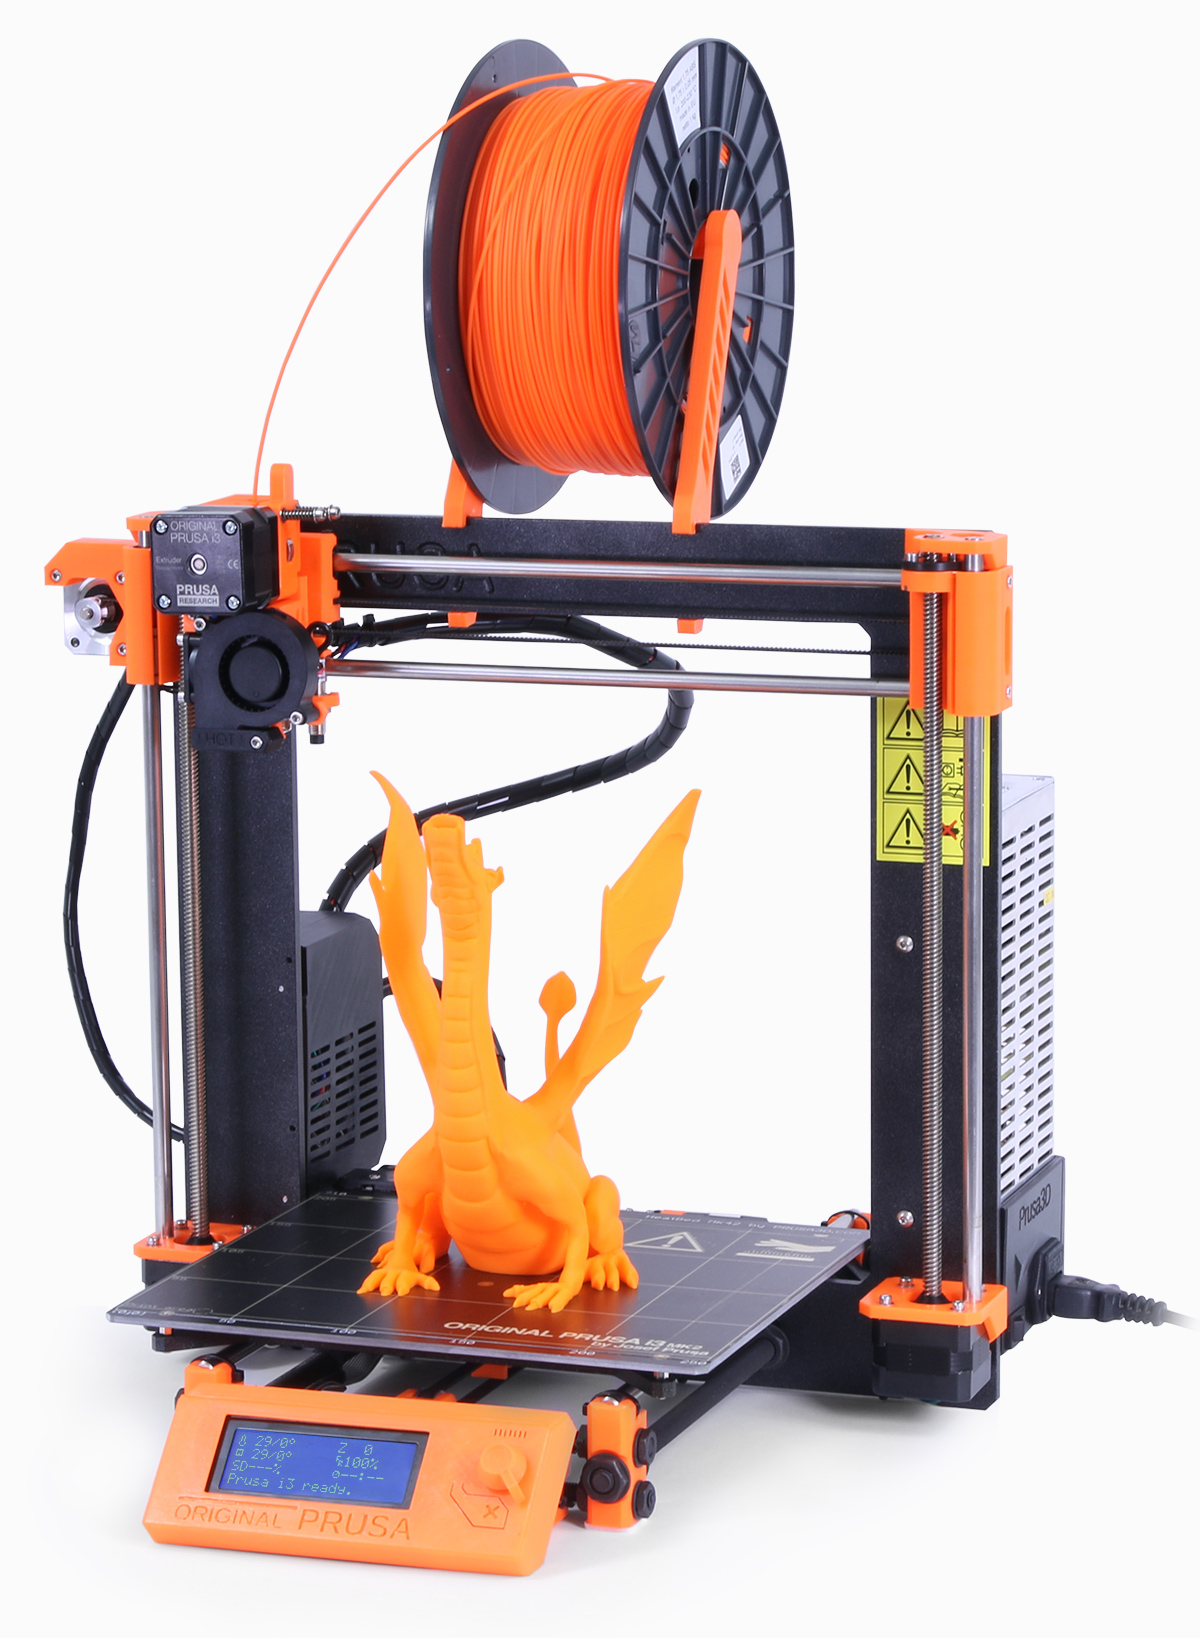
\includegraphics[width=7.5cm]{pics/Printer}
\caption{3D tiskárna Original Prusa i3 MK2}
\label{fig:PrinterMK2}
\end{center}
\end{figure}

\subsubsection{Trychtýřová anténa}
Jelikož bylo primárním cílem možnost použití produktu přímo bez post-processignu, je tedy nezbytné volit vodivé filamenty. Tyto materiály, jak již víme mají výrazně odlišné vlastnosti od jejich nosičů.

Pro námi navrženou anténu byly použity následující filamenty:
\begin{itemize}
\item Electrifi Conductive 3D Printing Filament
\item F-Electric Filament
\item Blackmagic 3D Conductive Graphene Filament
\item MKF Filament MKF-ABS F1.75 černá / VODIVÁ
\end{itemize}

Veškeré použité filamenty jsou na nosiči PLA, s vyjímkou MKF-ABS. Jako příměs jsou použity grafenové fragmenty (Blackmagic), uhlíkové nanotrubky (F-electric) a měďěné částice (Electrifi). Bohužel u materiálu MKF nebylo možné s dostatečnou přesností určit příměs jelikož výrobce tento údajneposkytuje. Podobná situace poté však ale platí i procentuální podíl příměsí, které jsou buďto tajné, či neznámé pro všechny testované vzorky.

Z hlediska vodivosti, tedy nejlepšího kandidáta na použití při realizaci dle udávaných parametrů (byly-li dostupné) je jednoznažně Electrify, který udává $16667\,S/m$. Nicméně je velmi důležitá jeho náročnost na tiskový proces vlivem velkého procenta mědi, která akumuluje teplo a značně prodlužuje zchlazení objektu pod teplotu skelného přechodu způsobující následnou deformaci tisknutého produktu vlivem gravitace.

Dalším významným faktorem filamenty Electrifi je jeho cena, $199.53\,CZK$/m. Pokud bychom tedy chtěli realizovat námi navržený trychtýř, bylo by nezbytné použít téměř 27\,m, celkem tedy $5 387\,CZK$ za předpokladu 100\,\% úspěšnosti realizace.

Jako reálnější materiály poté vychází F-electric, s vodivostí $133.33\,S/m$ a cenou $25.73\,CZK$/m, $694.71\,CZK$ za trychtýř, či Blackmagic, s vodivostí $166.67\,S$ a cenou $43.2\,CZK$/m, $1 166.4\,CZK$ za trychtýř, které vykazují výrazně vhodnější parametry pro tisk.

Před vlastní generací dat je však nutno vyrvořit profil charakterizující materiál z hlediska teplot, rychlosti procesu, chalzení, a ostatních parametrů. Pro získání prvnotního návrhu nastavení lze pouze převzít doporučené hodnoty výrobcem, nicméně ne vždy toto musí platit! Jelikož neexistuje jednotný standart pro 3D tiskrány typu: tiskový povrch, geometrie trysky, mechanika extruderu, a další, bude pravděpodobné že toto nastavení ve finální podobě bude odlišné.

\begin{figure}[h]
\begin{center}
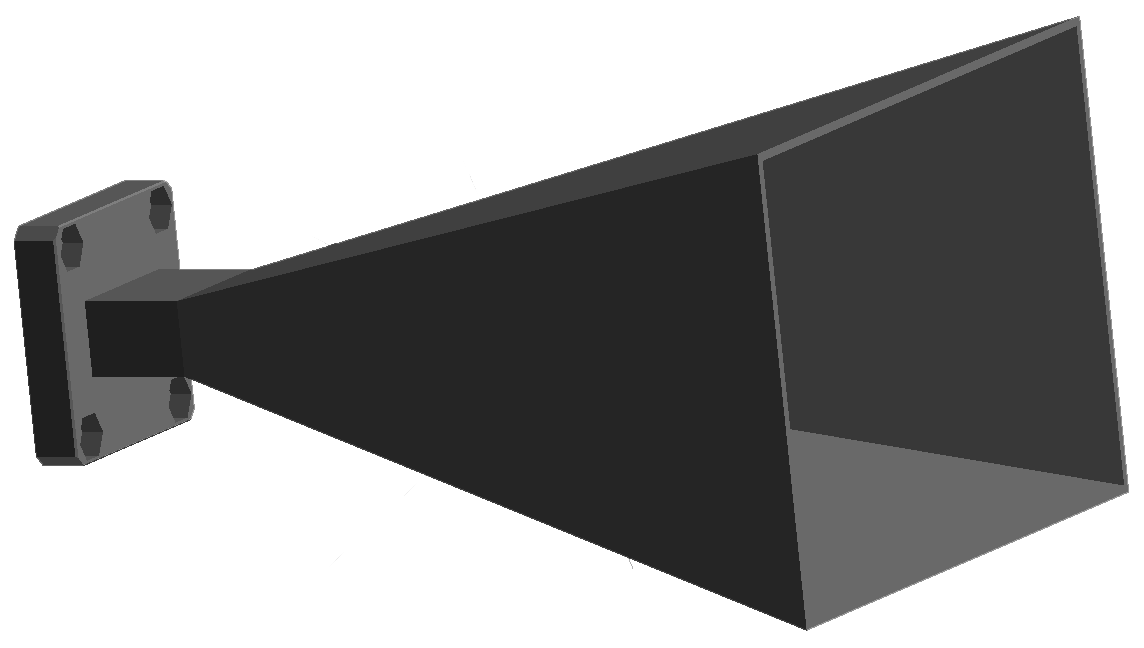
\includegraphics[width=9.5cm]{pics/HornFinal}
\caption{Výsledný model trychtýřové antény včetně příruby na vlnovod realizovaný technologií 3D tisku za použití F-electric filamentu}
\label{fig:HornRealFe}
\end{center}
\end{figure}

Bohužel však při realizaci dalších struktur docházelo k významným komplikacím znemožňující další produkci, zejména k ucpavání trysky \ref{fig:HornFail}.

K těmto skutečnostem pravděpodobně vedlo nadměrné hromadění příměsí v místě zužení trysky způsobující zúst mechanického odporu a nároků na potřebnou sílu k jeho překonání. Vlivem nízké mechanické soudržnosti materiálu a křehkosti způsobeno vysokým procentem plnění poté dochází k prokluzování podávacího mechanismu extruderu a následného výpadku extruze. Další pravděpodobnou příčinou mohl být vlastní průměr filamentu, který pokud je mimo specifikaci ($\pm$50\,$\mu$m) může dojít k podobné situaci jelikož ne vždy je možné protáhnout předmět větší než rozměry otvoru. 

Tyto komplikace byly částečně eliminovány použitím trysky $D_{nozzle} = 0.6\,mm$, avšak problémy stále přetrvávali a proces byl velmi nespolehlivý a neopakovatelný. Možné další principy eliminace mohou být realizovány například úpravou mechanické části extruderu, která by měla výrazně větší styčnou plochu podávacího mechanismu s filamentem pro možnost vyvinou vyšší tlačnou sílu.

\begin{figure}[h]
\begin{center}
\includegraphics[width=9.5cm]{pics/HornFail}
\caption{Důsledek ucpavání trysky v průběhu tisku modelu}
\label{fig:HornFail}
\end{center}
\end{figure}


\subsubsection{Anténní čočka}
Realizace anténní čočky je v porovnání s předchozím případem velmi zjednodušena z důvodu zvolení zpomalujícího typu, tedy použití dielektrického, nikoliv vodivého, materiálu.

Pro správnou funkci čočky a maximálnímu přiblížení se simulovaných modelů je důležité při generování dat pro technologický proces použít správný typ vnitřní struktury pro zajištění 100\.\% podílu dielektrického materiálu.

Pokud toto nebude při realizaci dodrženo, vlivem nehomogenního prostředí pro šíření vlny, obsahující mnoho velmi ostrých rozhraní vzduch/dielektrikum, způsobí velmi odlišné chování a pro jeho dostatečný popis je třeba k této struktuře přistupovat jako k metamateriálu.

Jelikož rozměry navržené čočky jsou natolik velké, že v kombinaci s vysokou teplotní roztažností materiálu a stoprocentním podílem materiálu v objektu, bylo nutné zvolit materiál PLA, případně PET z důvodu možného použití standartních tiskových nastavení s pouhou změnou procentuální výplně materiálem na 100\,\%.

\begin{figure}[h]
\begin{center}
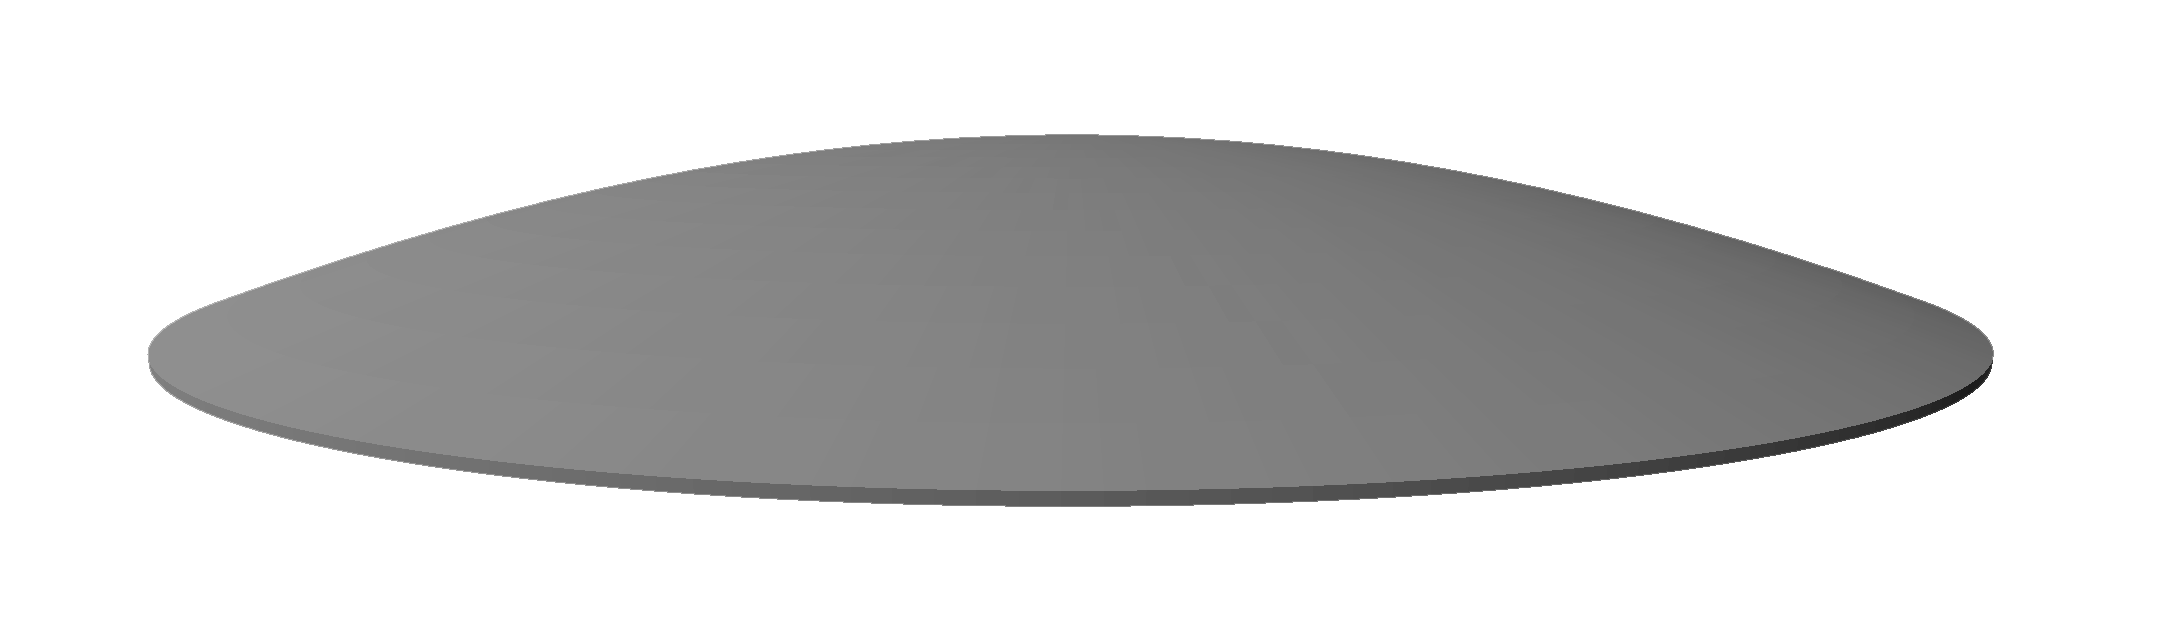
\includegraphics[width=9.5cm]{pics/LensModel}
\caption{Realizovaná anténní čočka z materiálu Plasty Mladeč PET transparent}
\label{fig:LensReal}
\end{center}
\end{figure}

\section{Pokovení}
Jelikož již dostupné vodivé filamenty disponují velmi malou vodivostí pro přímé použití, pro možnost následného pokovení však mohou být více než dostačující.

\subsubsection{Mokrá cesta}
Jako první cesta pro maximalizaci vodivosti produktu byla zvolena metoda elektricky vodivého laku EMI 35\cite{EMIdata}.

Použitý elektrický lak je založen na termoplastickém polymeru s přidaným speciálním měděným pigmentem rozpuštěném ve vhodné ředící složce. Po aplikaci laku v průběhu 24 hodin dojde k postupnému odpaření ředící složky a vznikne tenká vodivá vrstva, o tloušťce v řádu 50\,$\mu$m.

Při zvolení této cesty není nutno realizovat strukturu z vodivého polymeru jelikož přilnutí vodivé látky není podmíněno jeho vodivostí. Byl tedy zvolen materiál $Plasty Mladeč PET transparent$ z důvodu vhodných vlastností při tisku rozměrově blízkých k maximu použité 3D tiskárny.


\begin{figure}[h]
\begin{center}
%\includegraphics[width=9.5cm]{pics/HornFail}
\caption{Realizovaná struktura s následným nánosem EMI 25}
\label{fig:HornEMI}
\end{center}
\end{figure}

\subsubsection{Elektroformování}
Galvanoplastika je technologie známá a využívaná po mnoho desítek let. Jejím principem je elektroformování (z anglického „electroforming“) geometrických tvarů s využitím elektrochemického vylučování kovových povlaků na primární model. Využívá se principu elektrolýzy, avšak vylučovány jsou vrstvy v od desítek mikrometrů po jednotky milimetrů.\cite{Electroforming}.

Jelikož tato metoda je závislá na principu elektrolýzy, je nutné aby pokovovaný objekt vykazoval dostatečnou vodivost právě pro zajištění nutných podmínek vzniku. Toto může být například realizování například EMI 25 lakem, které mají však svá omezení. Pokud však vstupní vzorek již vykazuje vyšší vodivost, velmi se proces zjednoduší a není třeba využívat komplexních způsobů "zvodivení".

Pokud tedy realizujeme strukturu například z filamentu F-electric, který při prvních testech byl stoprocentně úspěšný, můžeme ji následně přímo pokovit elektroformováním.

Tento postup byl nejprve otestován v laboratorních podmínkách při prvotním testování před započatím této práce. Při výzkumu možností byla navržena základní mřížková struktura pro ověření použitelnosti metody. Dále pak bylo pozorováno velmi gradientní rozložení elektrického potenciálu, které řetězovou reakcí způsobylo nekonzistentní výsledné vrstvy s maximem u přípojného bodu elektrody.

Pro kompenzaci tohoto gradientního rozložení pole je možno využít postupné noření do lázně smeřem k přípojnému bodu za správné rychlosti.
\begin{figure}[h]
\begin{center}
\includegraphics[width=9.5cm]{pics/platingtest}
\caption{Výsledná testovací struktura s výraně viditělnou nekonzistentní vrstvou}
\label{fig:platingtest}
\end{center}
\end{figure}

Z důvodu toho, že se tento postup jevil jako velmi perspektivní, byla navázána spolupráce se společností Electroforming s.r.o. pro možnost využití produkčních zařízení za účelem pokovení realizované trychtýřové antény z materiálu F-electric.

Výsledkem této spolupráce byl velmi pozitivní z hlediska kvality a přilnavosti nanešené vrstvy (pomineme-li popsaná omezení technologie v 3.1 a přilnavost na hladké povrchy) a její vodivosti. Výsledná struktura při testu ohmického odporu standartním multimetrem CEM DT-61 vykazovala hodnoty pod rozlišovací schopnost.

Nicméně však vzhledem ke komunikačnímu šumu ve spolupráci, a nepředáním vzájemných znalostí pužitých technologíí došlo k deformaci výsledné struktury. Jelikož materiál použitý pro realizaci struktury disponuje teplotou skelného přechodu $\vartheta_g \simeq 50\,^\circ$$C$ a teploty lázní procesu pokovení tuto teplotu standartně přesahují. Na základě této zkušenosti byla varžena speciálně modifikovaná struktura, viz 3.1, bohužel však vlivem výše uvedených komplikací se ji již nepodařilo realizovat, to ale nevylučuje realizovatelnost, jen vyžaduje delší výzkum samotných materiálů.


\begin{figure}[h]
\begin{center}
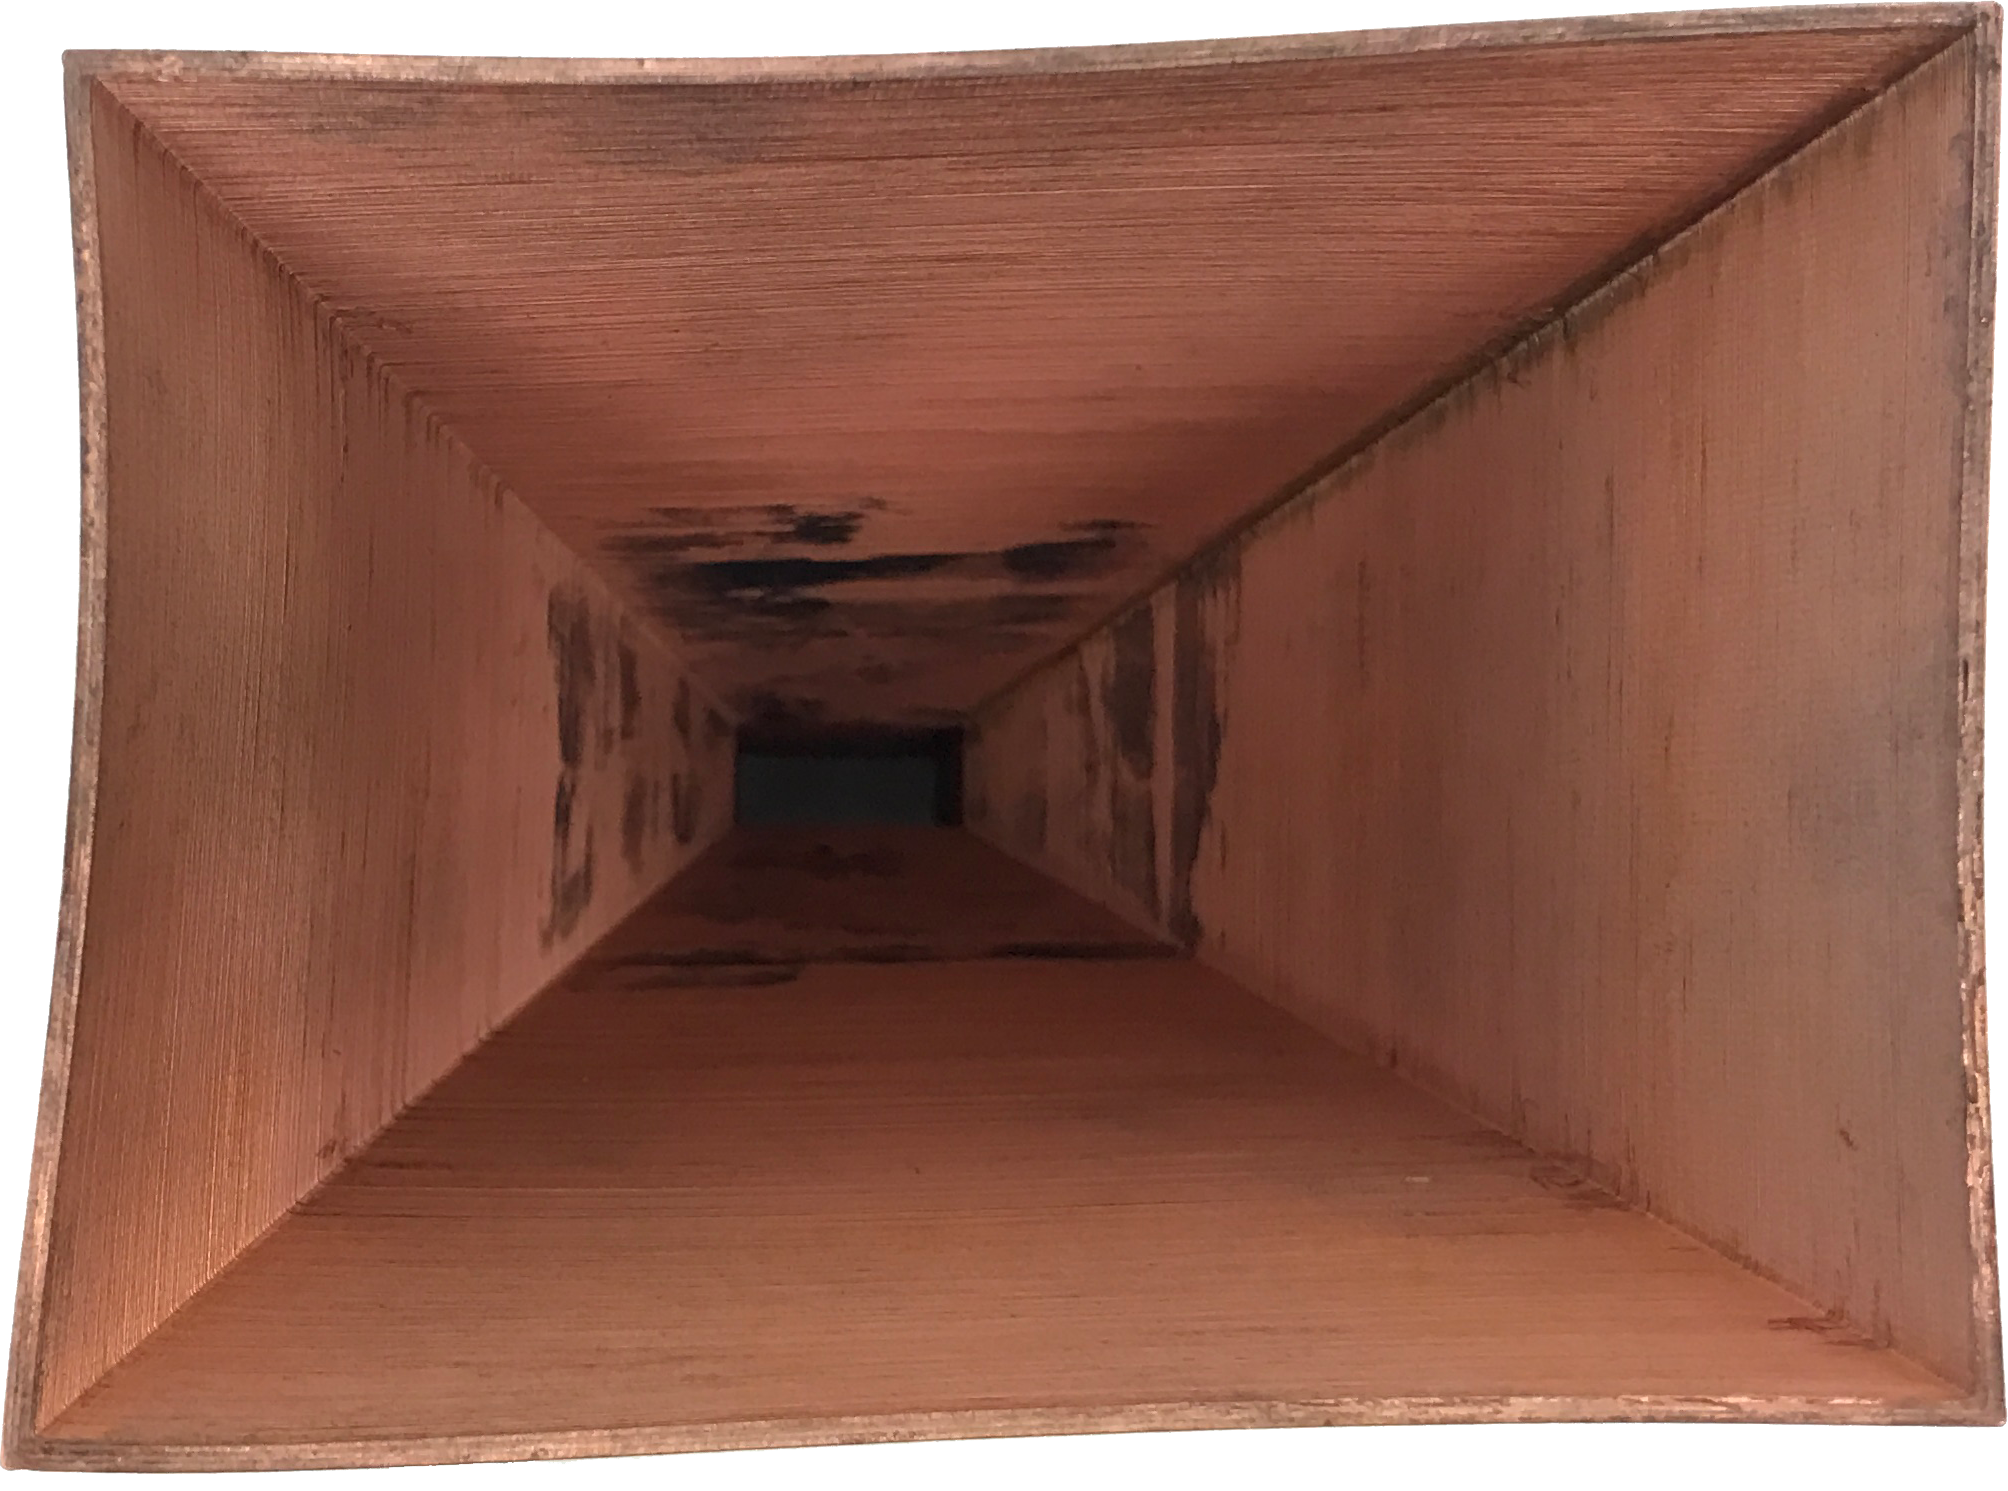
\includegraphics[width=9.5cm]{pics/plated/deform}
\caption{Deformace a nedokonalosti v dutině výsledné pokovené struktury}
\label{fig:PLdef}
\end{center}
\end{figure}

\begin{figure}[h]
\begin{center}
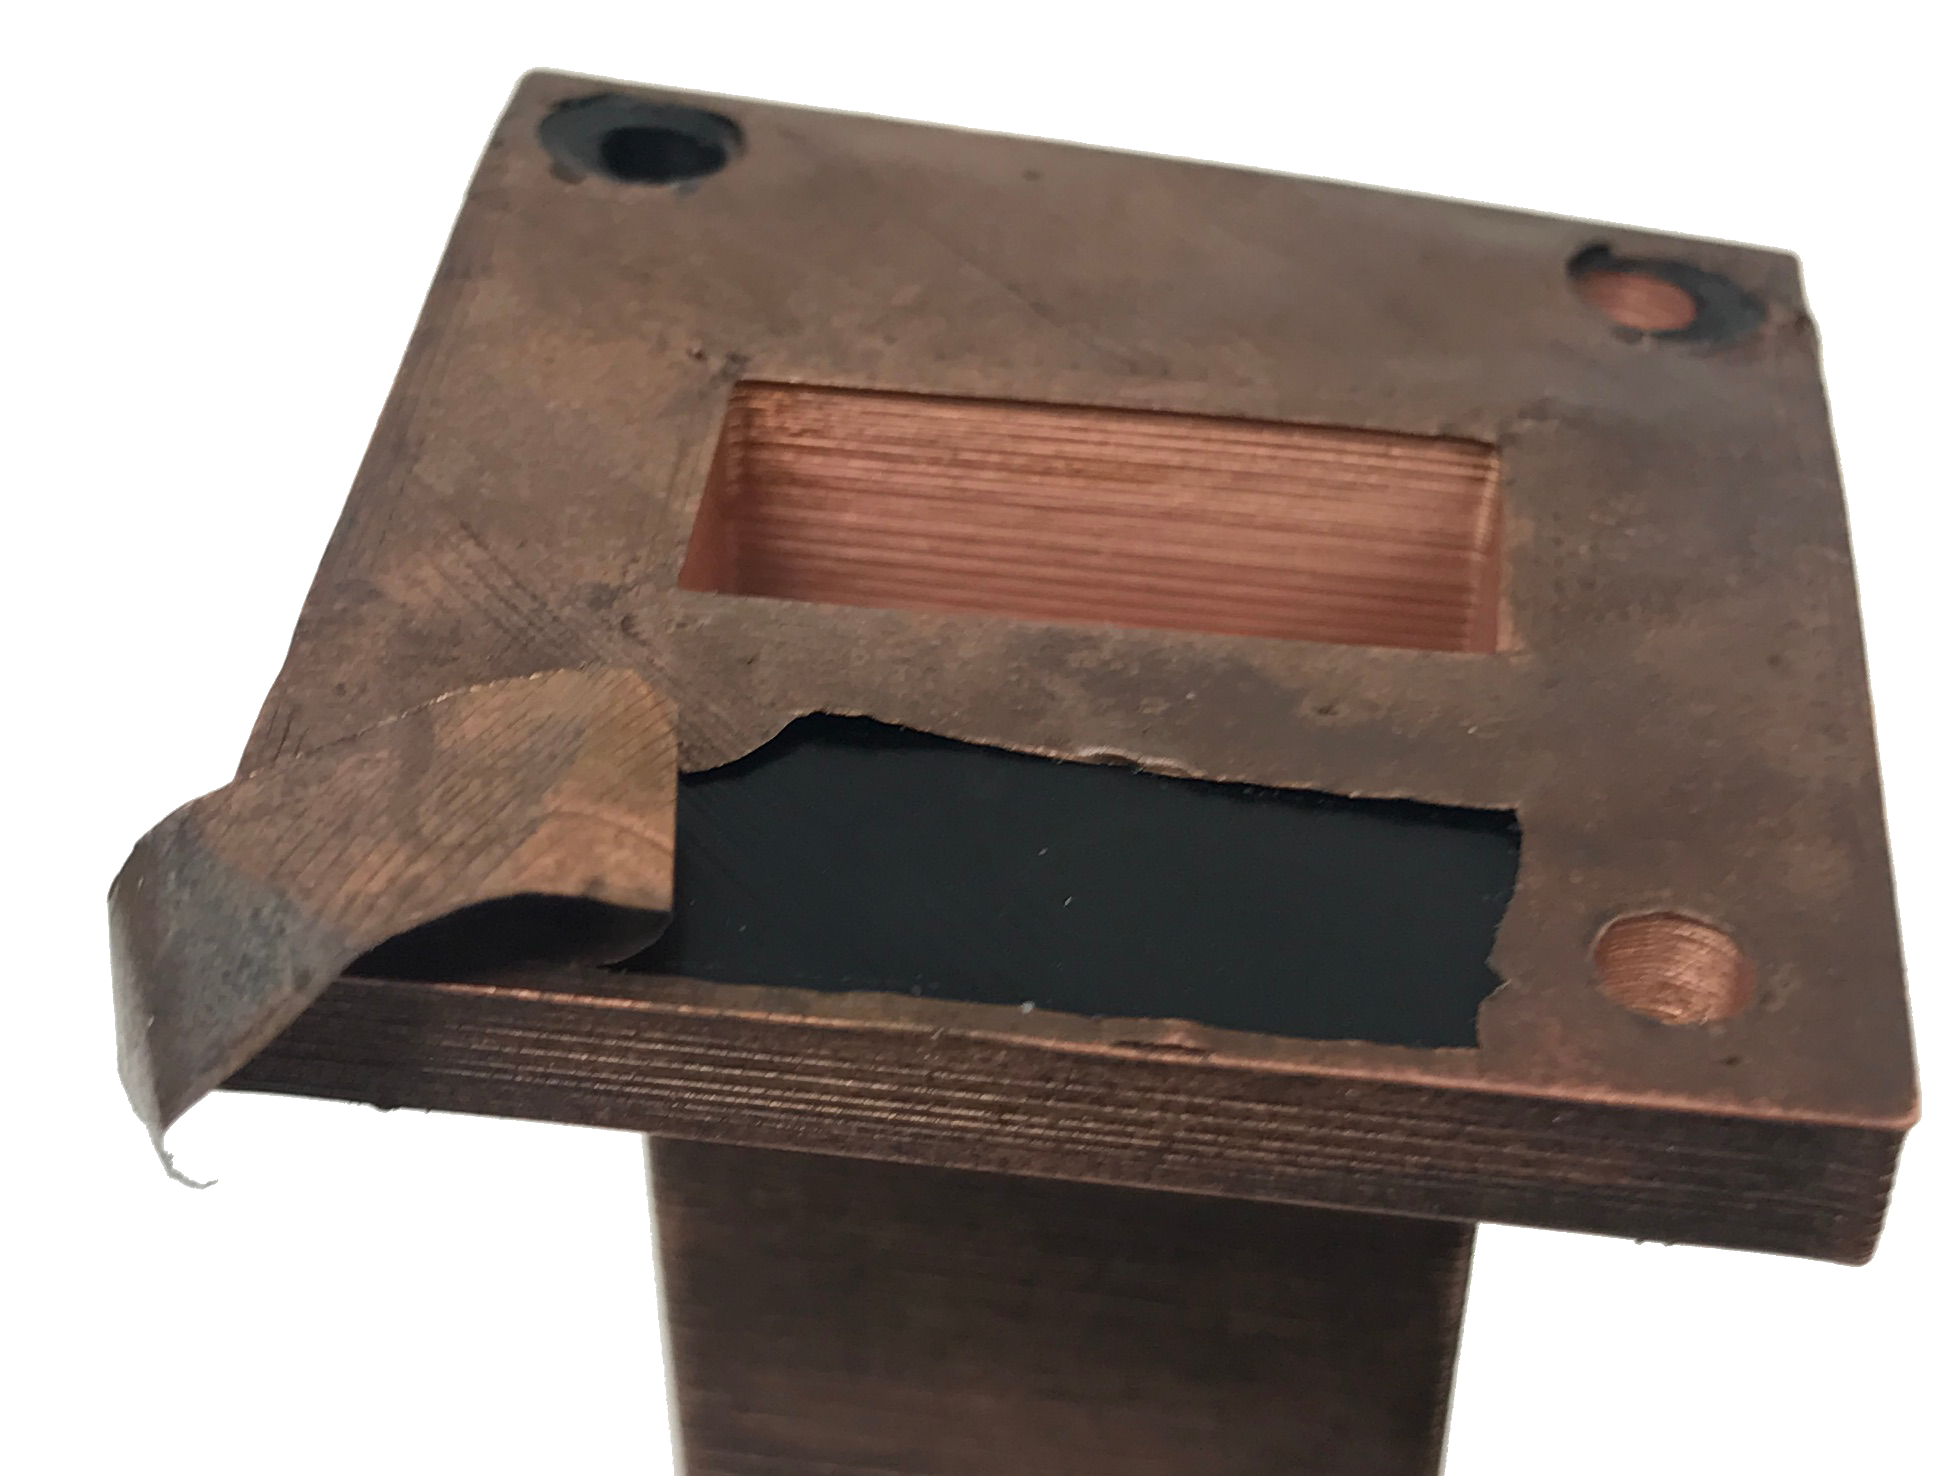
\includegraphics[width=9.5cm]{pics/plated/adhes}
\caption{Nízká přilnavost k hladkým povrchům}
\label{fig:PLadh}
\end{center}
\end{figure}


\section{Měření parametrů}
Realizované vzorky byly podrobeny dvojicí měření (impedančního přizpůsobení a vyzařovací charakteristiky) pro oveření funkčnosti a srovnání se simulací v CST MW studio.

\subsection{Impedanční přizpůsobení}
Pro měření impedančního přizpůsobení bylo využito standartní měřící metodiky za použití vektorového analyzátoru Rohde \& Schwarz ZVA67.

Blokové schéma měření je poté na \ref{fig:MatchDia}, kde \textbf{1}- Přechod z koaxiálního vedení na vlnovod R100, \textbf{2}- Kalibrační rovina, \textbf{3}- Měřená anténa.
\begin{figure}[h]
\begin{center}
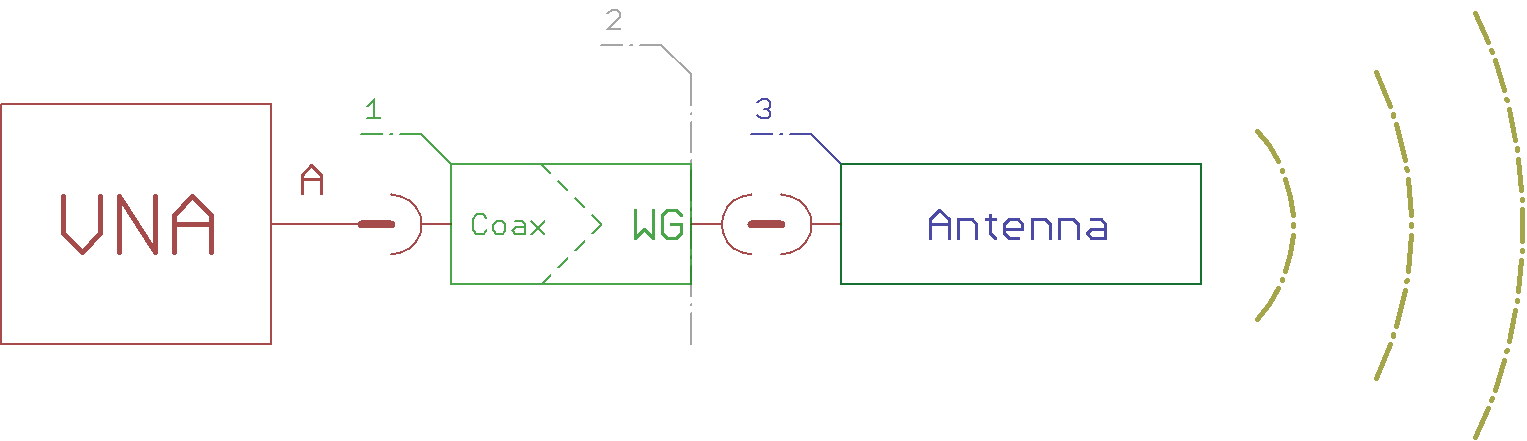
\includegraphics[width=9.5cm]{pics/MatchDia}
\caption{Blokové schéma měření impedančního přizpůsobení}
\label{fig:MatchDia}
\end{center}
\end{figure}

Před samotným měřením parametrů je velmi důležité zkalibrovat systém na vyznačené kalibrační rovině, tedy výstupu vlnovodného přechodu. Toto lze snadno udělat pomocí dvou kalibrů (zkratu, a definovaného úseku vlnovodu), kde za pomocí naměřených dat dojde ke spočítání korekce a následné nastavení kalibrační roviny.

Nutné však dodat, že pro měření definovaného úseku vlnovodu je nutno vlnovod ukončit opět přechodem na koaxiální vedení, ideálně identického od stejného výrobce, ze stejné série, a zapojit do druhého kanálu analyzátoru pro možnost změření charakteristiky úseku vedení v měřícím systému. 

\begin{figure}
\begin{tikzpicture}
\begin{axis}[
    xlabel={Angle /\,$^\circ$},
    ylabel={Amplitude /\,dB},
    minor tick num=10,
    minor grid style={gray!25},
    major grid style={black!50},
    xmin=8,xmax = 12,
    grid=both
]
\addplot [no markers, thick, blue] table [col sep=tab, y=AbsS11graph] {hornmatch.dat};
\addplot [no markers, thick, red] table [col sep=tab, y=AbsS11emi] {hornMatch.dat};
\legend{A,B};
\end{axis}
\end{tikzpicture}
\caption{Naměřené impedanční přizpůsobení realizované trychtýřové antény za použití \textbf{A} - F-electric, \textbf{B} - Plasty Mladeč PET transparent + EMI 25}
\label{fig:Matching}
\end{figure}

\subsection{Směrová charakteristika}
Druhým sledovaným parametrem realizovaných produktů byla směrová charakteristika, která byla v závislosti na dostupných technologiích měřena v anténní bezodrazné komoře pomocí automatizovaného měřícího systému NSI2000 pracující na principu uvedeném na schematu \ref{fig:DirectDia}. Kde 1 - Bezodrazná anténní komora, 2 - Rotační mechanismus (točna), CPU - Centrální procesní jednotka, VNA - Vektorový analyzátor, Room Controller - Řídící jednotka točny, R.A. - Známá vysílací anténa, A.U.T. - Měřená anténa, D - Vzdálenost antén.

\begin{figure}[h]
\begin{center}
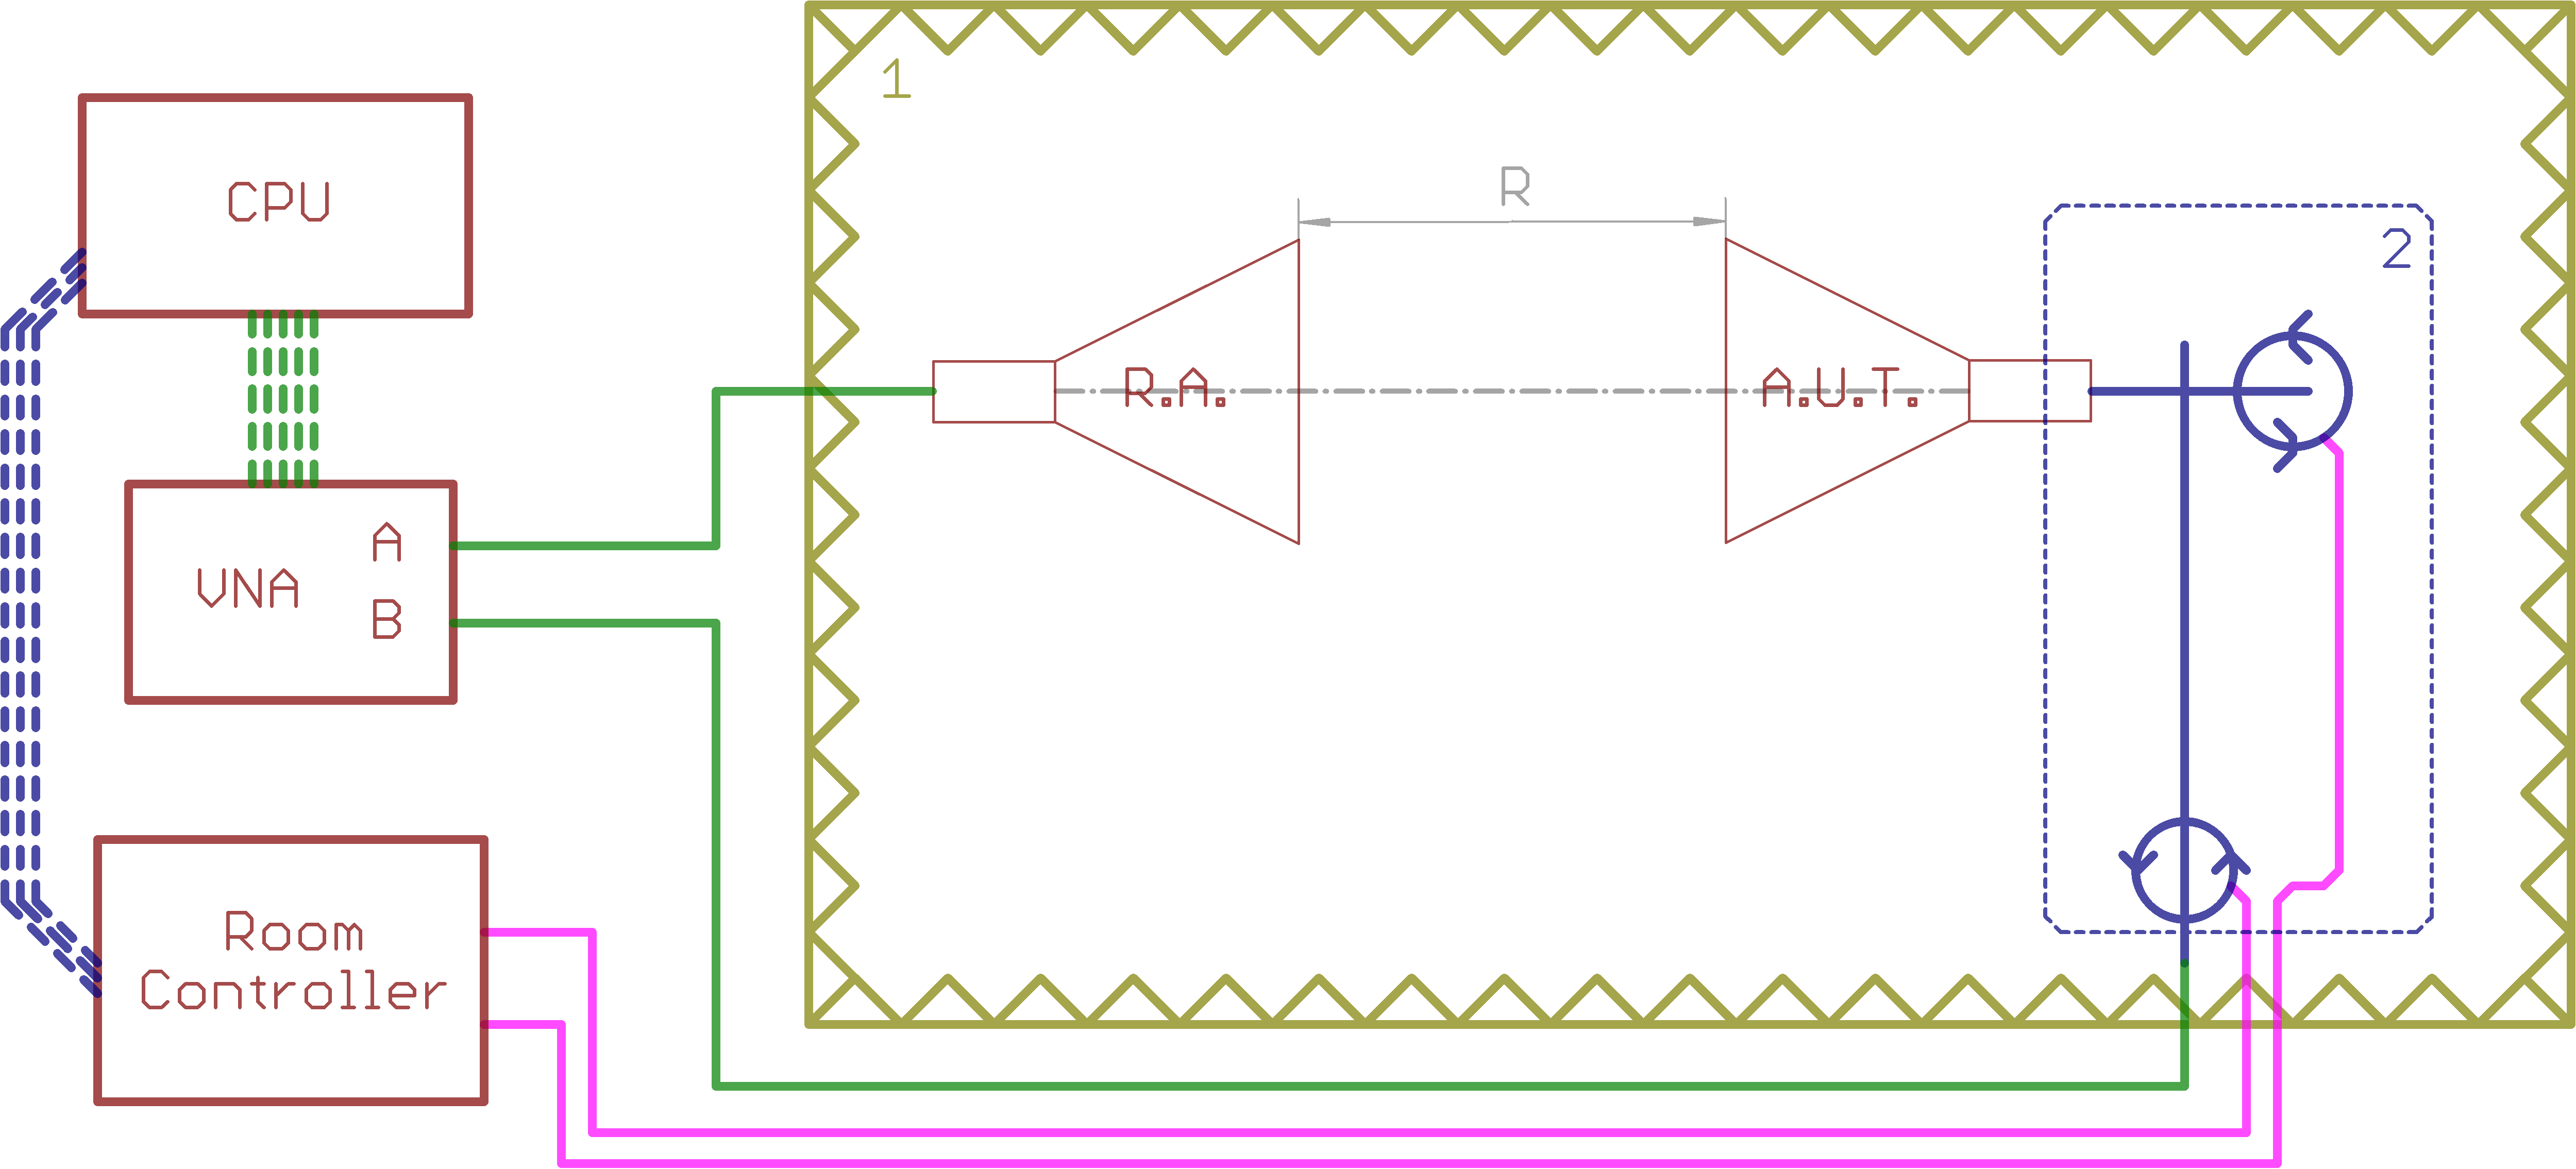
\includegraphics[width=9.5cm]{pics/DirectDia}
\caption{Zjednodušené blokové schéma měření směrové charakteristiky}
\label{fig:DirectDia}
\end{center}
\end{figure}

Skutečná realizace použité metody je však komplexnější, pro přiblížení metody je ale zjednodušený model dostačující.
Základní princip použité metody je založen na vysílání vlny známou anténou a její následné přijímání anténou testovanou za její postupné rotace kolem azimutu za stálého měření přijatého výkonu. Z naměřených hodnot (přijatého výkonu) poté pomocí známého Friisova vztahu \ref{eq:Friis} (kde $P_p$ - Přijatý výkon, $P_v$ - Vysílaný výkon, $G_v$ - Zisk vysílací antény, $G_p$ - Zisk měřené antény, $( \frac{\lambda}{4 \pi R} )^2$ - Ztráty volným prostorem) lze vypočítat zisk měřené antény v každém měřeném úhlu. Je však nutno zajistit, aby antény ležely v ose a v dostatečné vzdálenosti větší než vzdálená zóna, tedy $R \geq \frac{2\,D^2}{\lambda}$ (kde D je nevětší rozměr měřené antény a $\lambda$ vlnová délka), minimalizaci rušení z okolního prostředí a intenzitu odrazů v komoře.

\begin{equation}
P_p = P_v G_v G_p( \frac{\lambda}{4 \pi R} )^2
\label{eq:Friis}
\end{equation}

\begin{figure}
\begin{tikzpicture}[scale=1.4]
\begin{axis}[
    xlabel={Angle /\,$^\circ$},
    ylabel={Amplitude /\,dB},
    minor tick num=10,
    minor grid style={gray!25},
  	major grid style={black!50},
  	xmin=-180,xmax = 180,
  	ymin=-120, ymax=-60,
    grid=both
]
\addplot [no markers, thick, blue] table [col sep=tab, y=Ae-emi] {horn.dat};
\addplot [no markers, thick, red] table [col sep=tab, y=Ae-graph] {horn.dat};
\addplot [no markers, thick, green] table [col sep=tab, y=Ae-lens] {horn.dat};
\legend{F-electric, PET+EMI 25, F-electric+PET lens};
\end{axis}
\end{tikzpicture}
\label{fig:FarfieldsE}
\caption{Naměřené vyzařovací charakteristiky realizovaných trychtýřů v E rovině}
\end{figure}

\begin{figure}
\begin{tikzpicture}
\begin{axis}[
    xlabel={Angle /\,$^\circ$},
    ylabel={$P_p$ /\,dB},
    minor tick num=10,
    minor grid style={gray!25},
  	major grid style={black!50},
  	xmin=-180,xmax = 180,
  	ymin=-120, ymax=-60,
    grid=both
]
\addplot [no markers, thick, blue] table [col sep=tab, y=Ah-emi] {horn.dat};
\addplot [no markers, thick, red] table [col sep=tab, y=Ah-graph] {horn.dat};
\addplot [no markers, thick, green] table [col sep=tab, y=Ah-lens] {horn.dat};
\legend{F-electric, PET+EMI 25, F-electric+PET lens};
\end{axis}
\end{tikzpicture}
\label{fig:FarfieldsH}
\caption{Naměřené vyzařovací charakteristiky realizovaných trychtýřů v H rovině}
\end{figure}

\subsection{Extrakce parametrů}
Jak již bylo zmíněno, pro extrakci parametrů byla zvolena metoda transmisní/reflexní, viz blokové schéma \ref{fig:ExtractBlock}. Měření dat pro následnou spolehlivou extrakci je ale velmi obtížné realizovat se stoprocentní úspěšností prvního pokusu. Zejména z důvodu neznalosti parametrů materiálu (to je cílem celého snažení) a nutnosti splnit minimální 3\,dB útlum vložených vzorků do vlnovodu a zároveň respektovat omezení použité realizační technologie, fyzikální parametry materiálů a samozřejmě časovou náročnost.

Pro prvnotní měření byly zvoleny vzorky délek 49 a 69\,mm na základě dostupných vlnovodů pro splnění veškerých nutných podmínek za účelem získání použitelných výsledků. Jelikož však útlum nejdelšího vzorku byl naměřen v okolí 1.5\,dB z čehož lze odhadnout minimální délku vzorku 138\,mm. 

Upravené vzorky bohužel nemohli být realizovány v minimálních odhadovaných délkách a bylo nutné zvolit na základě dostupných úseků vlnovodu, pro finální realizaci tedy 149 a 199\,mm. Na základě těchto vzorků již bylo možné realizovat extrakci dielektrických parametrů, jelikož útlum ktrátkého úseku vykazoval útlum $>$3.5\,dB.

\begin{figure}
\begin{tikzpicture}
\begin{axis}[
    xlabel={Frequency /\,GHz},
    ylabel={Attenuation /\,dB},
    minor tick num=10,
    minor grid style={gray!25},
    major grid style={black!50},
    xmin=8,xmax = 12,
    ymin=-6, ymax=0,
    grid=both
]
\addplot [no markers, thick, red] table [col sep=tab, y=Apet149] {ParamExtract.dat};
\addplot [no markers, thick, orange] table [col sep=tab, y=Apet199] {ParamExtract.dat};
\addplot [no markers, thick, green] table [col sep=tab, y=Apla149] {ParamExtract.dat};
\addplot [no markers, thick, blue] table [col sep=tab, y=Apla199] {ParamExtract.dat};
\legend{PET 149\,mm,PET 199\,mm,PLA 149\,mm,PLA 199\,mm};
\end{axis}
\end{tikzpicture}
\label{fig:Attmeasure}
\caption{Naměřené útlumy vzorků pro extrakci parametrů}
\end{figure}

\begin{figure}
\begin{tikzpicture}
\begin{axis}[
    xlabel={Frequency /\,GHz},
    ylabel={$\real{\epsilon_r}$ /\,-},
    minor tick num=10,
    minor grid style={gray!25},
    major grid style={black!50},
    xmin=8,xmax = 12,
%    ymin=-6, ymax=0,
    grid=both
]
\addplot [no markers, thick, red] table [col sep=tab, y=EpsRePLA] {ExtractRes.dat};
\addplot [no markers, thick, blue] table [col sep=tab, y=EpsRePET] {ExtractRes.dat};
\legend{PLA, PET};
\end{axis}
\end{tikzpicture}
\label{fig:EpsReMeas}
\caption{Výsledky extrakce komplexní permitivity materiálů Plasty Mladeč transparent PLA a PET}
\end{figure}


\begin{figure}
\begin{tikzpicture}
\begin{axis}[
    xlabel={Attenuation /\,dB},
    ylabel={Loss tangent /\,-},
    minor tick num=10,
    minor grid style={gray!25},
    major grid style={black!50},
    xmin=8,xmax = 12,
%    ymin=-6, ymax=0,
    grid=both
]
\addplot [no markers, thick, red] table [col sep=tab, y=TgdPLA] {ExtractRes.dat};
\addplot [no markers, thick, blue] table [col sep=tab, y=TgdPET] {ExtractRes.dat};
\legend{PLA, PET};
\end{axis}
\end{tikzpicture}
\label{fig:TgdMeas}
\caption{Výsledky extrakce ztrátového činitele materiálů Plasty Mladeč transparent PLA a PET}
\end{figure}


